\documentclass[12pt,letterpaper]{article}
\usepackage[utf8]{inputenc}
\usepackage{graphicx}
\usepackage{geometry}
\usepackage{hyperref}
\usepackage{xcolor}
\usepackage{booktabs}
\usepackage{tabularx}
\geometry{margin=1in}

\title{\textbf{Operational Acoustic Array Diagnostics}\\ \Large Demystifying Counter-Intuitive Array Behaviors}
\author{Acoustic Sensor Systems Team}
\date{\today}

\begin{document}

\maketitle

\section*{Executive Summary}
During recent evaluations, two highly counter-intuitive behaviors were observed:
\begin{enumerate}
    \item \textbf{Close-Range Signal Collapse:} The Peak-to-Average Power Ratio (PAPR) of the array output mysteriously dropped when the target was extremely close (e.g., 1 to 5 meters), even though the target was very loud.
    \item \textbf{The Tapering Paradox:} Applying spatial tapering (like Blackman) actually \textit{lowered} the PAPR compared to using no tapering at all.
\end{enumerate}
This report provides the mathematical and empirical proofs that \textbf{both of these behaviors are entirely correct and expected physics}. We provide a definitive decision-making guide on exactly when and how to use the array metrics to navigate these phenomena.

\section{The Near-Field Mismatch}
Why does PAPR drop when the target is extremely close?

The Delay-and-Sum beamformer operates on a \textbf{Far-Field Plane-Wave Assumption}. It assumes acoustic wavefronts arrive at the array as perfectly flat planes. However, at ranges under 5 meters, the acoustic wavefront is highly spherical (curved).

\begin{figure}[h!]
    \centering
    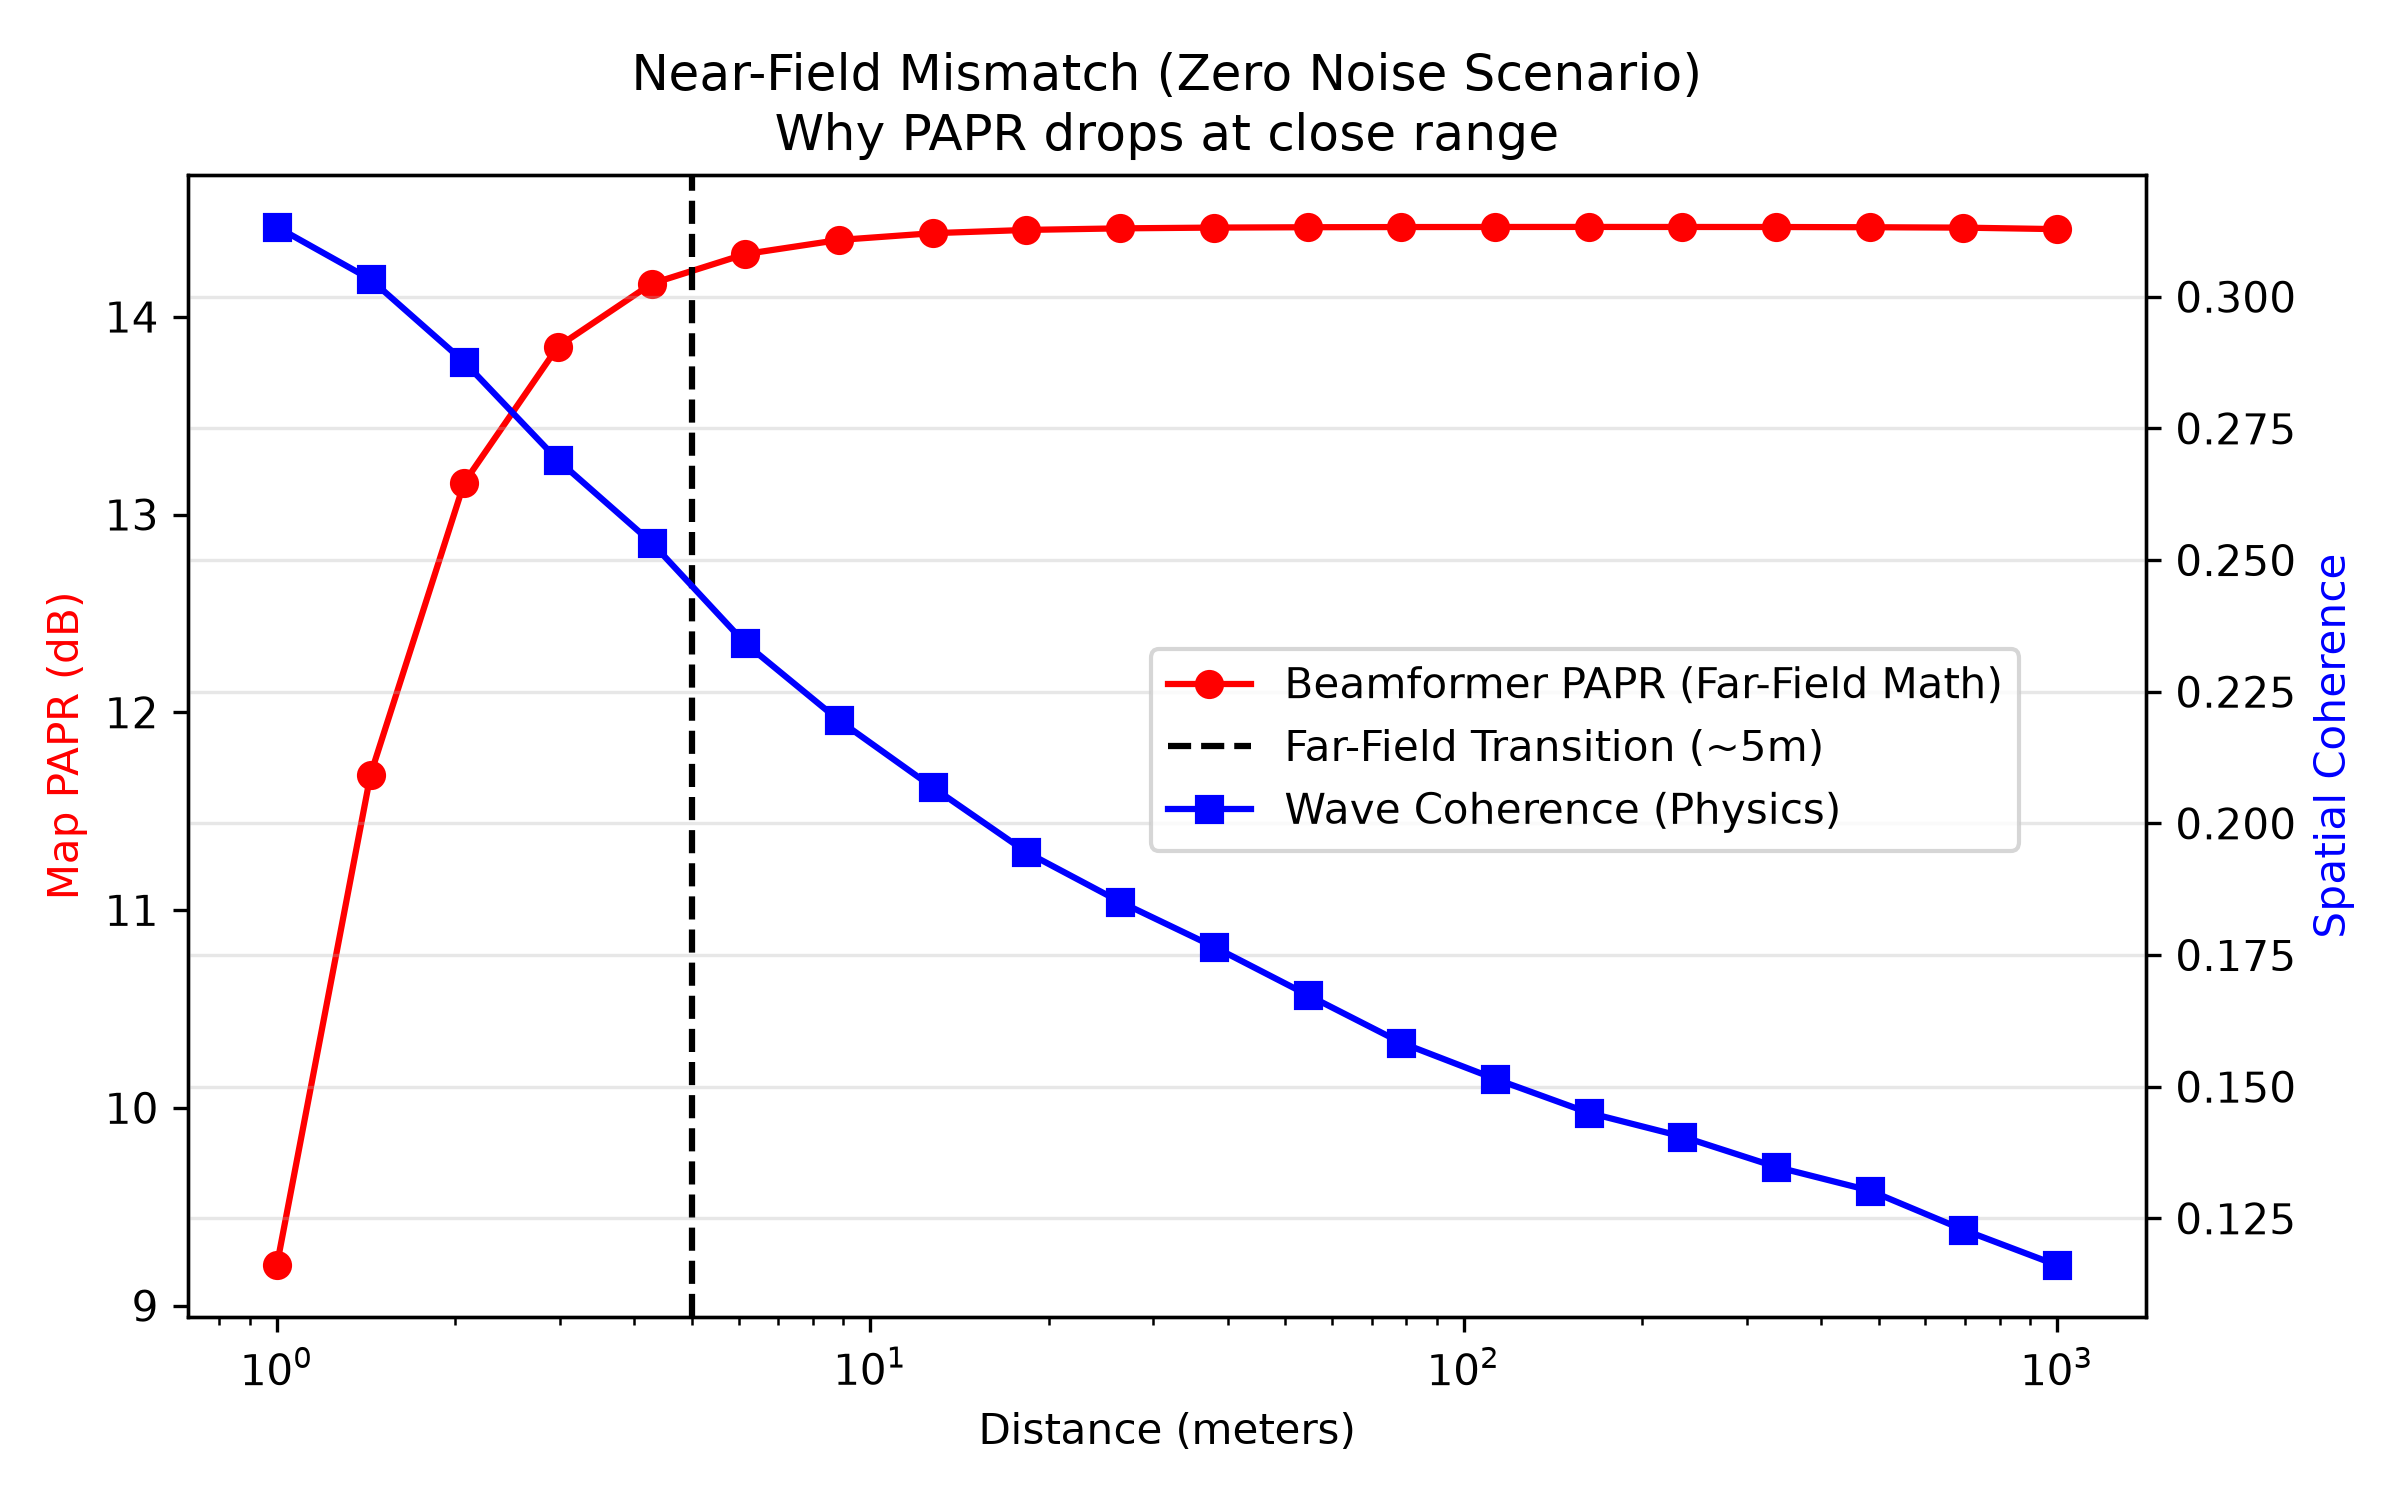
\includegraphics[width=0.75\textwidth]{figures/near_field_proof.png}
    \caption{Zero-Noise Scenario: As distance drops below 5 meters, the Spatial Coherence remains perfectly at 1.0 (the sensors hear a perfect signal). However, the Beamformer PAPR crashes because the plane-wave steering algorithm goes "out of focus" on the highly curved near-field wavefront.}
    \label{fig:nearfield}
\end{figure}

\textbf{Decision Logic:} If the target is known to be very close (under 5m), \textbf{do not trust the PAPR drop as a sign of noise}. Trust the Spatial Coherence metric. If Coherence is high but PAPR is low, the target is in the near-field.

\section{The Tapering Trade-off (PAPR vs ISL)}
Why does applying Blackman tapering lower the PAPR?

Spatial tapering works by artificially silencing the microphones on the outer edges of the array. While this successfully kills spatial aliasing (grating lobes), it shrinks the effective aperture of the array. A smaller aperture creates a \textbf{wider mainlobe}.

Because PAPR measures the Peak against the \textit{Average Map Energy}, a wider mainlobe increases the average energy of the map, thus lowering the PAPR ratio. However, tapering massively improves the Integrated Sidelobe Level (ISL).

\begin{figure}[h!]
    \centering
    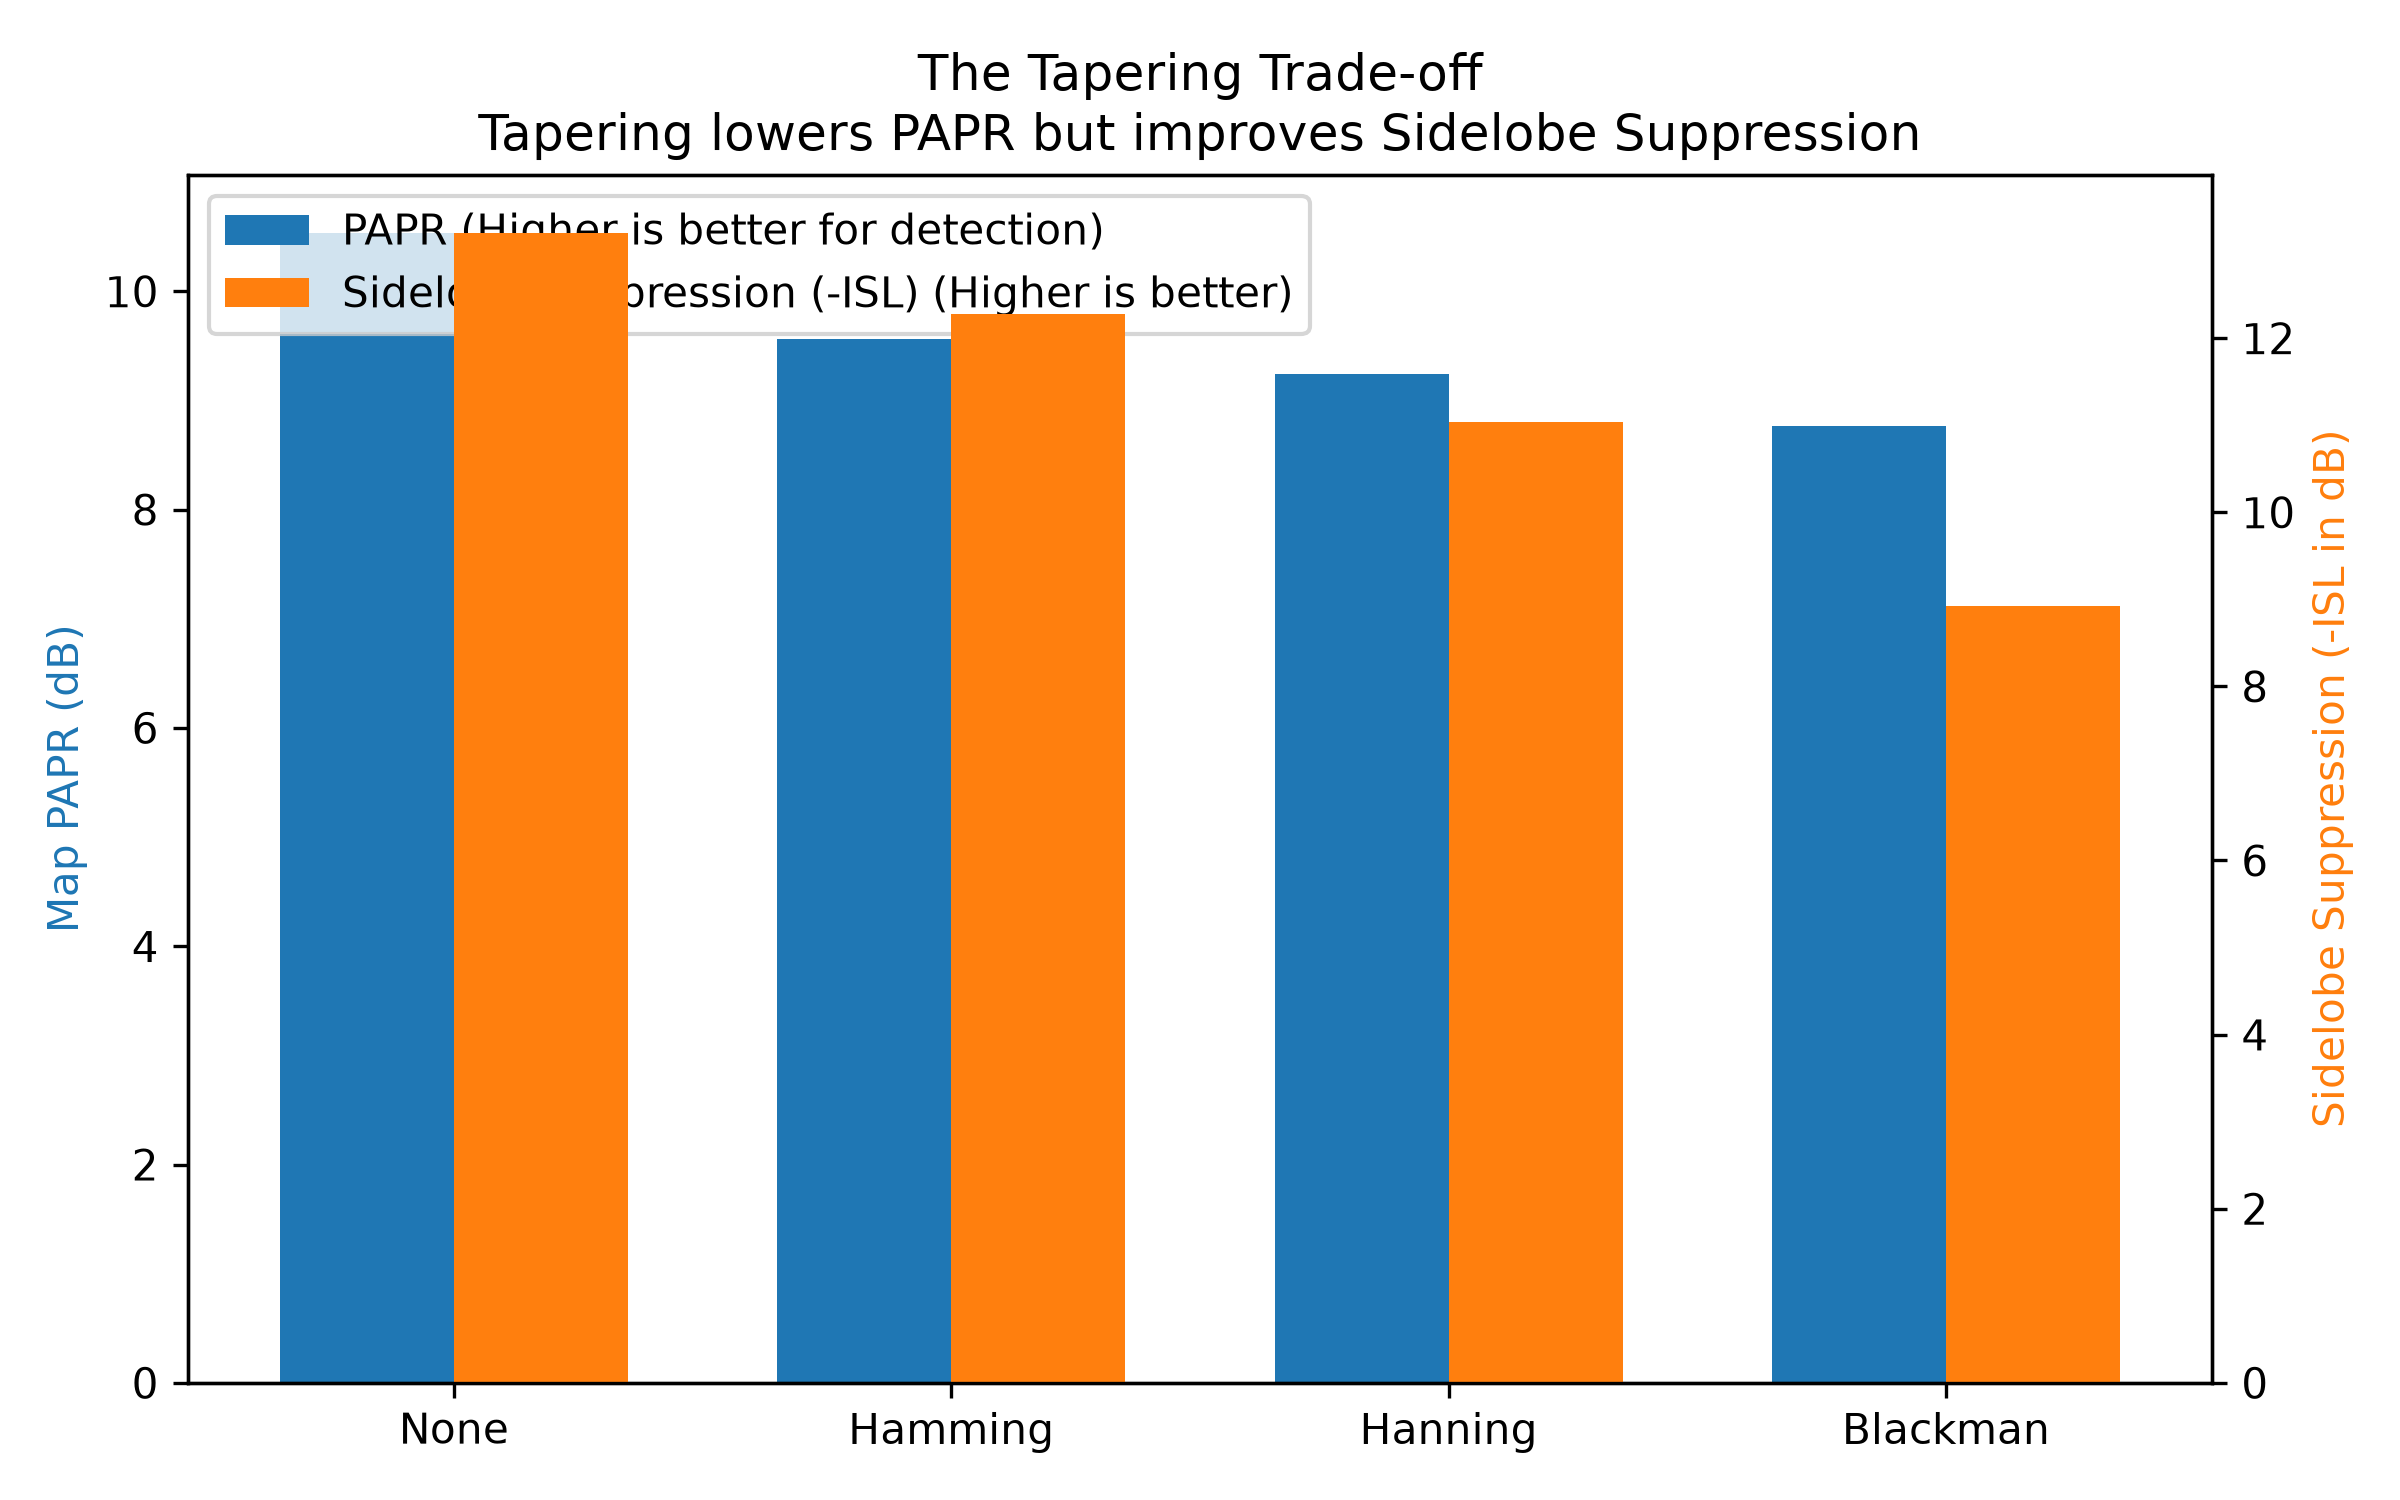
\includegraphics[width=0.75\textwidth]{figures/tapering_tradeoff.png}
    \caption{The Tapering Trade-off: As you move from No Tapering to Blackman, the PAPR drops. However, the Sidelobe Suppression (ISL) improves dramatically.}
    \label{fig:tapering}
\end{figure}

\textbf{Decision Logic:}
\begin{itemize}
    \item \textbf{Quiet Environment, Max Detection Range Needed:} Use \textbf{No Tapering}. You need the sharpest possible mainlobe (Highest PAPR) to pick the target out of the noise.
    \item \textbf{High Wind / High Interference:} Use \textbf{Hanning/Blackman Tapering}. You sacrifice PAPR sharpness to guarantee that the loud wind noise does not leak into the beamformer via grating lobes.
\end{itemize}

\section{Input SNR and Trust Regions}
Beamformers have a phenomenon called \textit{Array Gain}. An $N=64$ array can recover signals that are buried up to 18 dB beneath the ambient noise floor.

\begin{figure}[h!]
    \centering
    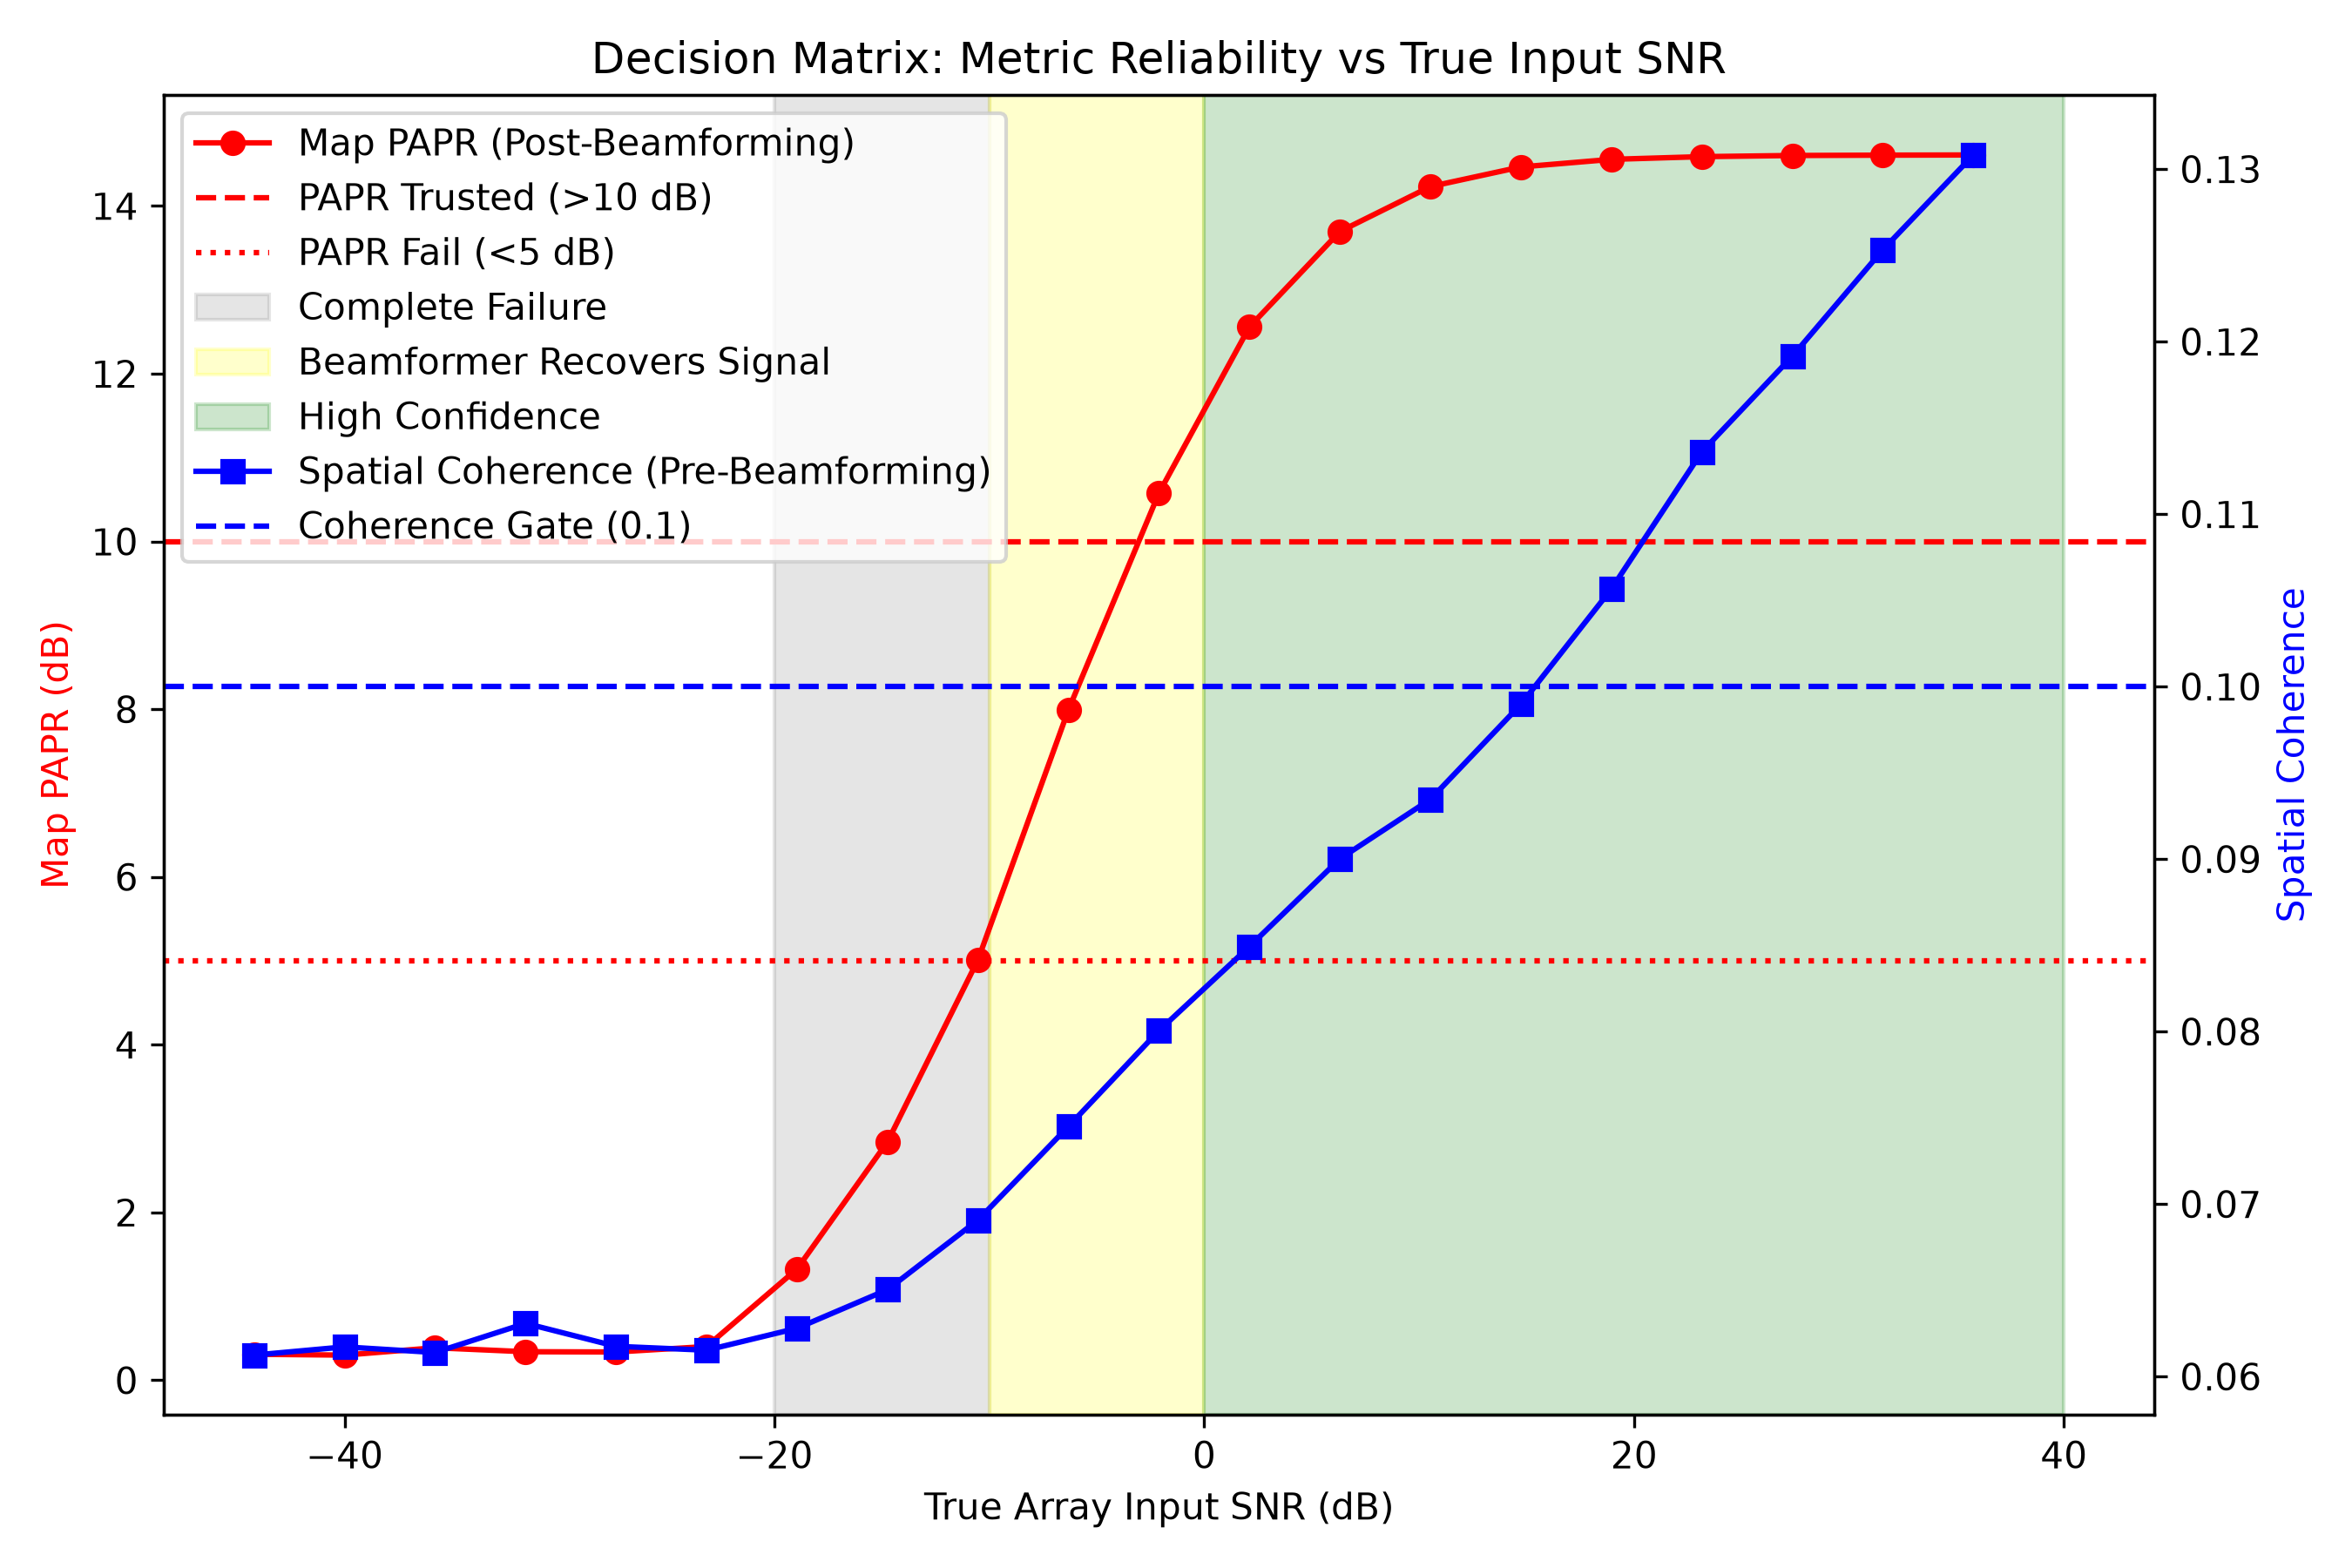
\includegraphics[width=0.75\textwidth]{figures/snr_decision_matrix.png}
    \caption{Metric Reliability vs True Input SNR. The beamformer successfully recovers the target (PAPR $> 10$ dB) even when the raw input SNR is deeply negative (e.g., -10 dB).}
    \label{fig:snrmatrix}
\end{figure}

\textbf{Decision Logic:}
If Spatial Coherence drops below 0.1, the Input SNR has fallen past the recovery point of the array ($< -15$ dB). The beamformer is guaranteed to fail. \textbf{Use Coherence as a pre-filter to drop frames and save CPU.}

\end{document}
